\section{Modelo Conceitual}
\label{sec:conceitual}

O modelo conceitual descreve \emph{o que} o sistema guarda, sem decidir
\emph{como}. Ele usa a notação de Chen, no estilo do brModelo: as entidades
ficam em retângulos, os relacionamentos em losangos e os atributos em
círculos, com o identificador em preto. A cardinalidade (mín, máx)
junto de uma entidade diz quantas instâncias dela se ligam a
\emph{uma} instância da outra ponta. Em \emph{assina}, por exemplo, o
(1,n) junto de Usuário diz que todo plano tem ao menos uma pessoa, e o
(0,n) junto de Plano diz que uma conta pode existir sem plano.

\begin{figure}[htbp]
  \centering
  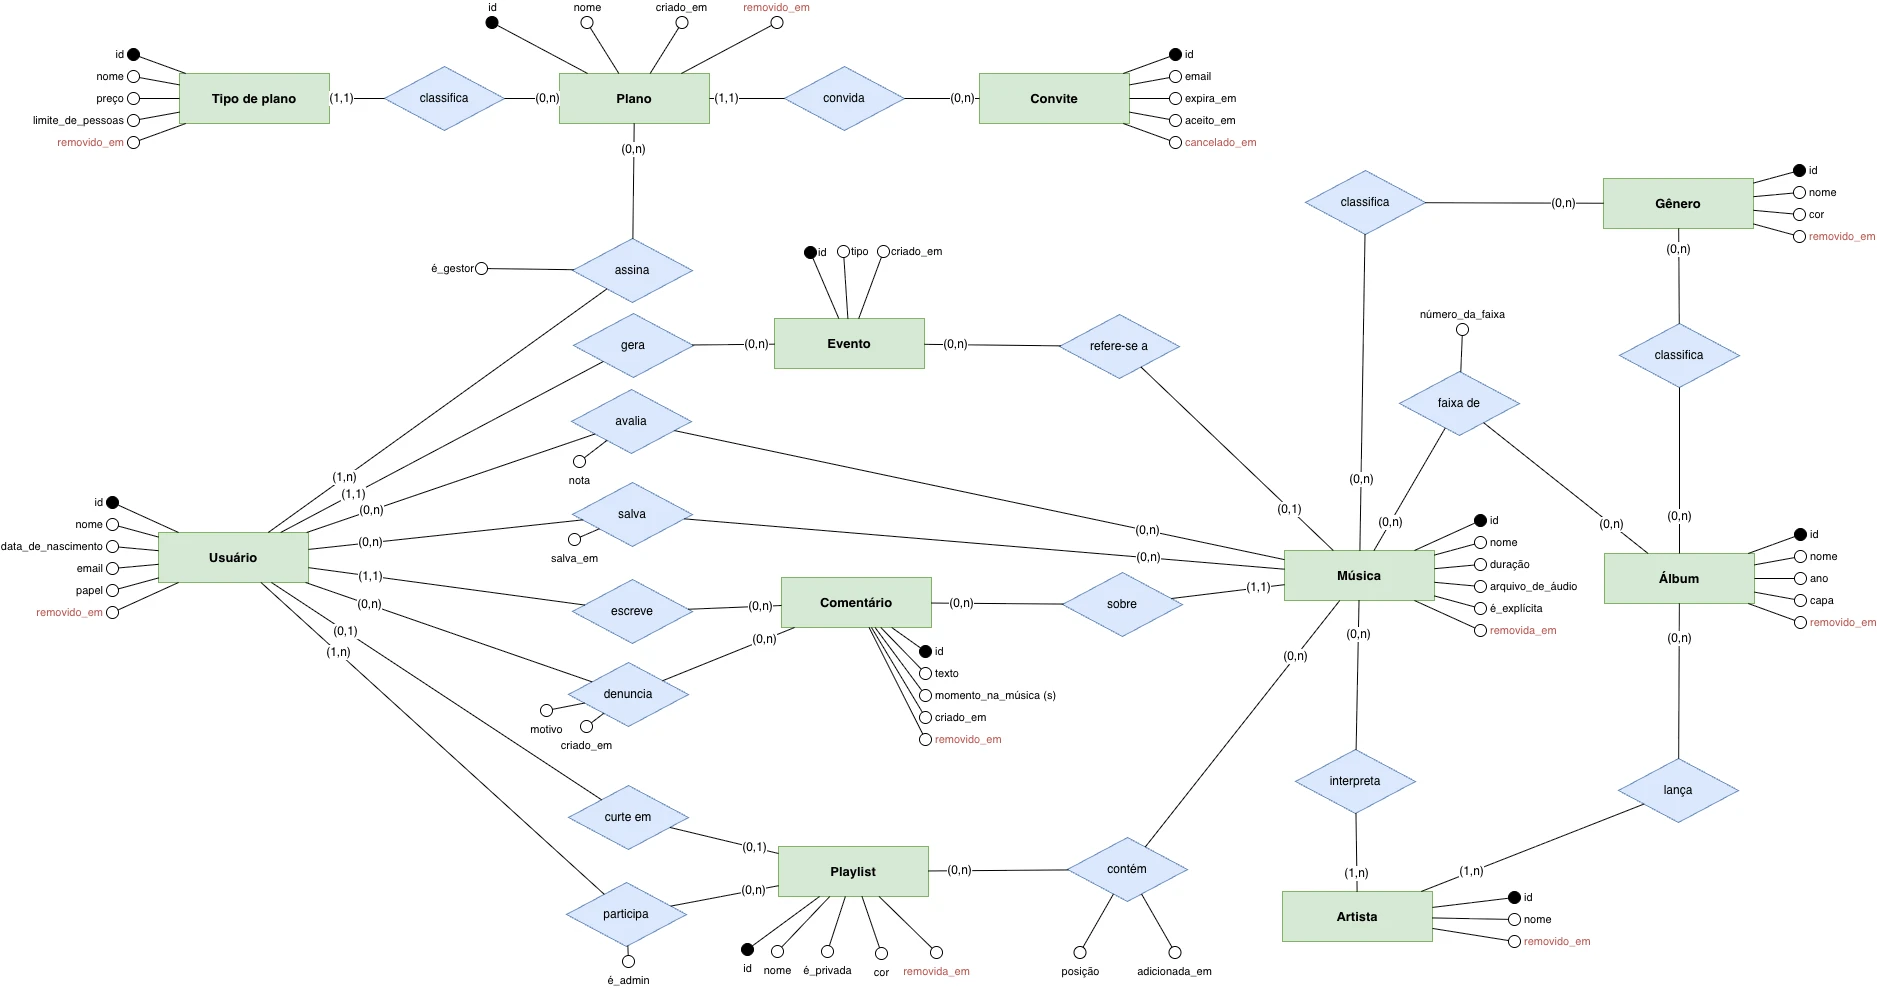
\includegraphics[width=\textwidth]{figuras/der-conceitual.png}
  \caption{Diagrama Entidade-Relacionamento conceitual do Zovic}
  \label{fig:der}
\end{figure}

Como o diagrama é conceitual, ele não mostra chaves estrangeiras nem tabelas
associativas. Um relacionamento é desenhado uma única vez, pela linha que liga
as entidades. Quando o vínculo tem dados próprios, eles aparecem como
atributos do losango: a \emph{nota} pertence a \emph{avalia}, e não ao usuário
nem à música; a \emph{posição} de uma faixa pertence a \emph{contém}, porque a
mesma música ocupa posições diferentes em playlists diferentes.

\subsection{Entidades}

\begin{table}[htbp]
  \centering
  \caption{Entidades do modelo conceitual}
  \label{tab:entidades}
  \begin{tabularx}{\textwidth}{@{}L{0.55}L{1.45}@{}}
    \toprule
    \poliCabTabela{Entidade} & \poliCabTabela{O que representa} \\
    \midrule
    Usuário & Uma conta. O papel (\emph{admin} ou \emph{assinante}) define o que ela pode fazer; o visitante não tem conta e não aparece no banco. A data de nascimento decide se a conta vê conteúdo explícito. \\
    Tipo de plano & Uma oferta comercial, com preço e limite de pessoas: Individual (1) e Família (4). \\
    Plano & Uma assinatura de um tipo de plano. \\
    Convite & Um convite do gestor para alguém entrar no plano familiar, com validade. \\
    Música & Uma faixa do catálogo, com duração, arquivo de áudio e a marca de conteúdo explícito. \\
    Álbum & Um lançamento, com ano e capa. \\
    Artista & Quem interpreta músicas e lança álbuns, com foto opcional. \\
    Gênero & Uma classificação de músicas e álbuns, com uma cor para a interface. \\
    Playlist & Uma lista ordenada de músicas, pública ou privada, com capa opcional. \\
    Comentário & Um texto sobre uma música, que pode apontar um momento dela (em segundos). \\
    Evento & Um registro de uso: cadastro, login, logout, reprodução, pulo ou música ouvida. \\
    \bottomrule
  \end{tabularx}
\end{table}

\FloatBarrier
\subsection{Relacionamentos}

\begin{table}[htbp]
  \centering
  \caption{Relacionamentos, cardinalidades e atributos}
  \label{tab:relacionamentos}
  \small
  \begin{tabularx}{\textwidth}{@{}L{0.85}L{1.2}L{0.45}L{1.5}@{}}
    \toprule
    \poliCabTabela{Relacionamento} & \poliCabTabela{Entidades} & \poliCabTabela{Tipo} & \poliCabTabela{Atributos e regras} \\
    \midrule
    classifica & Tipo de plano -- Plano & 1:N & Todo plano tem exatamente um tipo \\
    assina & Usuário -- Plano & N:M & \emph{é\_gestor}; todo plano tem ao menos uma pessoa \\
    convida & Plano -- Convite & 1:N & Todo convite é de um plano \\
    gera & Usuário -- Evento & 1:N & Todo evento é de uma conta \\
    refere-se a & Evento -- Música & N:1 & Opcional: só eventos de reprodução têm música \\
    avalia & Usuário -- Música & N:M & \emph{nota}, de 1 a 5 \\
    salva & Usuário -- Música & N:M & \emph{salva\_em} \\
    escreve & Usuário -- Comentário & 1:N & Todo comentário tem um autor \\
    sobre & Comentário -- Música & N:1 & Todo comentário é de uma música \\
    denuncia & Usuário -- Comentário & N:M & \emph{motivo}, \emph{criado\_em}; uma denúncia por pessoa e comentário \\
    participa & Usuário -- Playlist & N:M & \emph{é\_admin}; toda playlist tem ao menos um membro \\
    curte em & Usuário -- Playlist & 1:1 & A playlist ``Músicas Curtidas'' de cada conta \\
    contém & Playlist -- Música & N:M & \emph{posição}, \emph{adicionada\_em} \\
    faixa de & Música -- Álbum & N:M & \emph{número\_da\_faixa} \\
    interpreta & Artista -- Música & N:M & Toda música tem ao menos um artista \\
    lança & Artista -- Álbum & N:M & Todo álbum tem ao menos um artista \\
    classifica & Gênero -- Música & N:M & -- \\
    classifica & Gênero -- Álbum & N:M & -- \\
    \bottomrule
  \end{tabularx}
\end{table}

\FloatBarrier
\subsection{Decisões de modelagem}

\paragraph{Remoção lógica.} Músicas, álbuns, artistas, gêneros, playlists,
planos, usuários, comentários e avaliações nunca são apagados de verdade.
Removê-los preenche o atributo \emph{removido\_em}, destacado em vermelho na
\cref{fig:der}. Isso preserva o histórico: uma música tirada do catálogo
continua contando nas estatísticas de reprodução, e o email de uma conta
removida continua reservado.

\paragraph{Dados derivados ficam de fora.} O modelo não guarda o que pode ser
calculado a partir de outros dados. A média das notas de uma música sai de
\emph{avalia}, e o número de reproduções sai dos eventos. Guardar esses valores
numa coluna criaria redundância: os dois números poderiam divergir. O mesmo
vale para os totais do sistema (usuários, músicas e playlists), que um
\campo{COUNT} já calcula.

\paragraph{Autenticação é infraestrutura.} As sessões, as credenciais e os
tokens de verificação existem porque o Better Auth precisa deles, e não por
uma regra do negócio. Eles aparecem no modelo relacional, mas não no
conceitual.
